
\documentclass[12pt]{article}
\usepackage{amsmath}
\usepackage{graphicx}
\usepackage{amssymb}

\title{Estimating Dynamics of the Brain from Neuron Recordings}
\author{Abhinav Muraleedharan}
\date{October 21, 2023}

\begin{document}

\maketitle

\section{Introduction}

The brain, as a complex dynamical system, governs a diverse range of behaviors and cognitive processes, presenting a fundamental challenge in neuroscience. Unraveling the dynamics of the brain holds the key to understanding the neural mechanisms underlying these processes. Beyond modeling neural activity, elucidating how such activity correlates with an organism's behavior is crucial for developing Brain-Computer Interfaces, clinical treatments for conditions like epilepsy, depression, and other neurodegenerative diseases. \\

%%%% give an overall overview of existing approaches
Machine learning techniques have played a pivotal role in modeling brain dynamics, and modeling the correlation between neural dynamics and behavior of an animal. In \cite{pandarinath2018inferring}, Pandarinath et al. introduced LFADS, an RNN-based method to infer latent dynamics from neural data.  More recently, transformer-based models\cite{vaswani2017attention, geneva2022transformers}, have been applied to learn neural dynamics and behaviour model. In \cite{ye2021representation}, Pandarinath et al applied transformer-based models to learn neural dynamics without an explicit dynamical model. While LFADS and NDT (Neural Data Transformers) were focused on learning neural dynamics from single trial recordings, Azabou et.al recently introduced POYO \cite{azabou2023unified}, a transformer-based model to learn neural dynamics from multi-session neural recordings.
\\

Although transformer-based models have shown remarkable success in general language modelling tasks and more recently in learning population dynamics of neurons, they exhibit poor scaling properties especially when applied to neural spiking data. Furthermore, unlike text data, neural recording probes sample on the order of kHz, and hence are characterized by high temporal resolution. This unique temporal aspect of neural spiking data presents a challenge for transformers, which are originally designed for sequential data but may struggle with the high-frequency nature of neural signals. The transformer's poor scaling properties become particularly evident when recording from a large number of neurons simultaneously, as the number of potential firing patterns exponentially increases with the number of neurons.
\\

In this work, we introduce a new class of autoregressive models to overcome limitations imposed by the architecture of attention-based transformer models. Our model has an unbounded context length and hence can capture long-range dependencies in the time series dataset. Furthermore, the complexity of training and inference of the parametrized model is independent of the context length, and hence our approach is computationally more efficient when compared to transformer-based autoregressive models.







\section{Method}
\subsection{Problem Description}
Imagine we are recording data from $D$ neurons distributed across different regions of the brain. Let $x(t_i) \in \mathbb{R}^D$ denote the observed neural activity at timestep $t_i$ and let $y_i$ denote the observed behaviour of the animal at timestep $t_i$. From the time series dataset $\mathcal{D} = \{(x_i,y_i,t_i) \}_{i=1}^N$ of neural recordings, our goal is to
construct:
\begin{itemize}
    \item A predictive model of underlying brain dynamics
    \item A probabilistic model to predict behaviour of the organism at time $t+1$ given brain recordings until timestep $t$.
\end{itemize}
More formally, let's assume that the spiking activity is generated by an underlying non-stationary stochastic process defined by $p_t(x)$. 
\begin{equation}
    x(t) \sim p_t(x)
\end{equation}
The probability of observing a sequence of neural recordings and behavior can be expressed as:
\begin{equation}
    p( \{x_1,y_1\},\{x_2,y_2\},\{x_3,y_3\},..) = 
    \lim_{N \to \infty} \prod_{i=1}^{N} p(\{x_{i},y_{i}\}| \{x_1,y_1\},\{x_2,y_2\},..\{x_{i-1},y_{i-1}\})
\end{equation}
In the context of neural recordings, it is convenient to assume that the neural recording data and behavior can be modelled with separate probability distributions of the form:
\begin{equation}
   \prod_{i=1}^{N} p_d(\{x_{i}\}| \{x_1\},\{x_2\},..\{x_{i-1}\})
\end{equation}
\begin{equation}
   \prod_{i=1}^{N} p_b(\{y_{i}\}| \{x_1\},\{x_2\},..\{x_{i-1}\})
\end{equation}
Specifically, we assume that that the neural observed neural spiking data at timestep $t_i$ is not dependent on the behavior variables in the preceding timesteps. Probability distributions of this nature have been extensively investigated in the field of language modeling. In conventional autoregressive frameworks, the approximation of conditional distributions often involves the utilization of parameterized models constrained by a finite context limit\cite{vaswani2017attention}. While autoregressive models of this kind have been extremely successful in generating plausible language \cite{radford2018improving}, they still struggle to capture long-range dependencies due to the finite context length limit\cite{hahn2020theoretical}. Furthermore, the complexity of training and inference of transformer-based models is $\mathcal{O}(N^2)$, where $N$ is the context length of the transformer model.\\




\subsection{Approach}

First, we introduce a convolution operation to construct a random variable $ \zeta_k $ from a sequence of random variables $\{x_i\}_{i=1}^{k- 1}$. Mathematically, we define $ \zeta_k $ as:
\begin{equation}
    \zeta_i = \sum_{k=1}^{i-1} 2^{-k} \sigma_{\theta}(x_{i-k}) 
\end{equation}
Here, $x_k \in \mathbb{R}^D$ is the observed neural activity at timestep $t_k$, and $\sigma_{\theta}: \mathbb{R}^D \rightarrow \{0,1\}^D $ is a thresholding function, where $\sigma_{\theta}(x_i^{j}) = 1, \forall x_i^{j} > \theta $. (We use the notation $x_i^{j}$ to denote $j$ th element of the vector $x_i$.)
\\

Now, note that $\zeta_k $ has a recursive property, specifically:
\begin{equation}
    \zeta_{i+1} = 2^{-1}\zeta_i +  2^{-1}\sigma_{\theta}(x_i)
\end{equation}
Now, we approximate the conditional distribution defined in eq(3) with 
\begin{equation}
   \prod_{i=1}^{N} p_d(\{x_{i}\}| \{x_1\},\{x_2\},..\{x_{i-1}\}) 
   \approx  \prod_{i=1}^{N} p_d(\{x_{i}\}|\zeta_i)
\end{equation}
To learn the dynamics of the brain from neural recordings in an unsupervised manner, we maximize the following likelihood:
\begin{equation}
    \mathcal{L}(X,\theta) = \sum_i log(p_d(\{x_{i}\}|\zeta_i;\theta))
\end{equation}
Here, $X = \{x_1,x_2,....x_M\}$, the dataset of neural recordings. \\

Note that in this approach, the context window is not bounded, and the complexity of learning the parametrized model $p_d(\{x_{i}\}|\zeta_i;\theta)$ is independent of the length of the context window. While training the model, we apply eq(6) to recursively update $\zeta_i$ in an online fashion, instead of pre-computing and storing $\{\zeta_i\}_{i=1}^N$ separately.
 \\

 To learn the correlation between neural dynamics and behavior, we follow a similar approach and approximate the conditional distribution defined in eq(4) with:
\\
 \begin{equation}
   \prod_{i=1}^{N} p_b(\{y_{i}\}| \{x_1\},\{x_2\},..\{x_{i-1}\}) 
   \approx  \prod_{i=1}^{N} p_b(\{y_{i}\}|\zeta_i)
\end{equation}
We define the loss function associated with this approach as the negative log-likelihood of the observed behavioral outcomes given the estimated neural activity states. Formally, the loss function \( \mathcal{L} \) is expressed as:

\[
\mathcal{L}(X,Y,\phi) = -\sum_{i} \log p_b(\{y_i\}|\zeta_i;\phi)
\]



\section{Data:}
\subsection{ Two-Photon Recording Data}
Two-photon microscopy is a powerful imaging technique widely used in neuroscience research to capture detailed neuronal activity in living organisms with high spatial resolution ~\cite{svoboda2006principles}.\\

A typical two-photon recording setup involved using a specialized microscope capable of imaging neural activity in real-time (See Fig(1)). This enables us to record the activity of individual neurons in the cortex during various experimental conditions, providing valuable insights into the spatiotemporal patterns of neural firing. 
\begin{figure}[htbp] % You can adjust the placement options (htbp) as needed
  \centering
  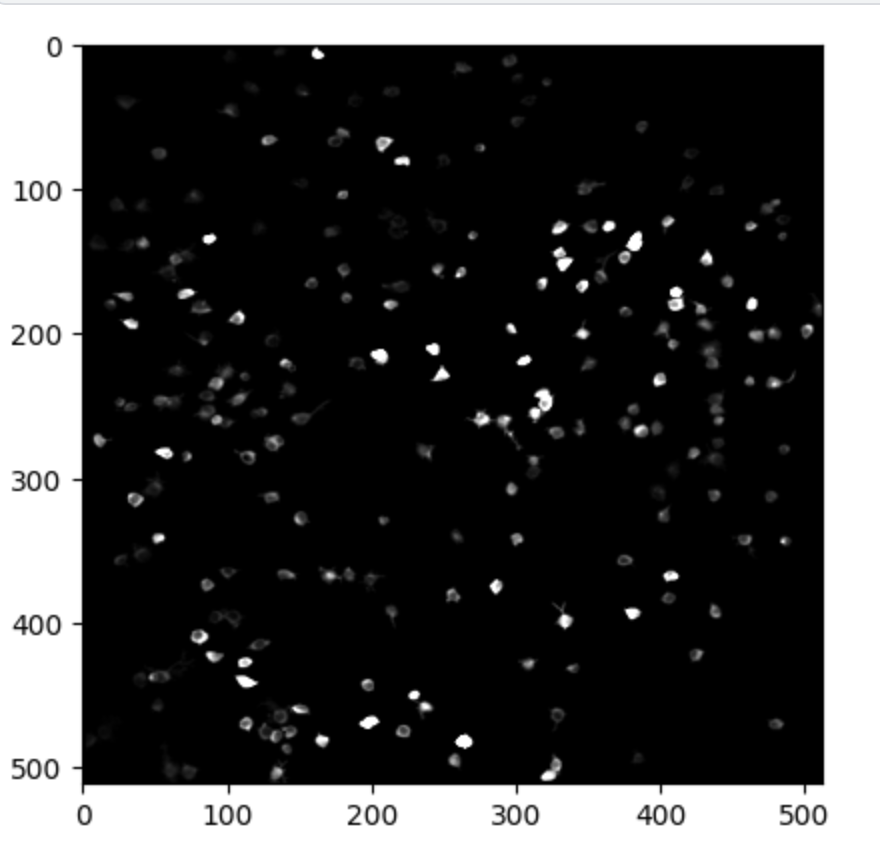
\includegraphics[width=0.75\linewidth]{neuropixel.png}
  \caption{Two Photon Recording data }
  \label{fig:your-label}
\end{figure}

\subsection{Inferred Neural Activity from Neuropixel data}
From the neuropixel data, specific neurons can be located and spike activity over time can be inferred using image processing algorithms. The neuronal spiking activity is not a smooth signal (See Figure 2), and hence is qualitatively different from other time series datasets. 

\begin{figure}[htbp] % You can adjust the placement options (htbp) as needed
  \centering
  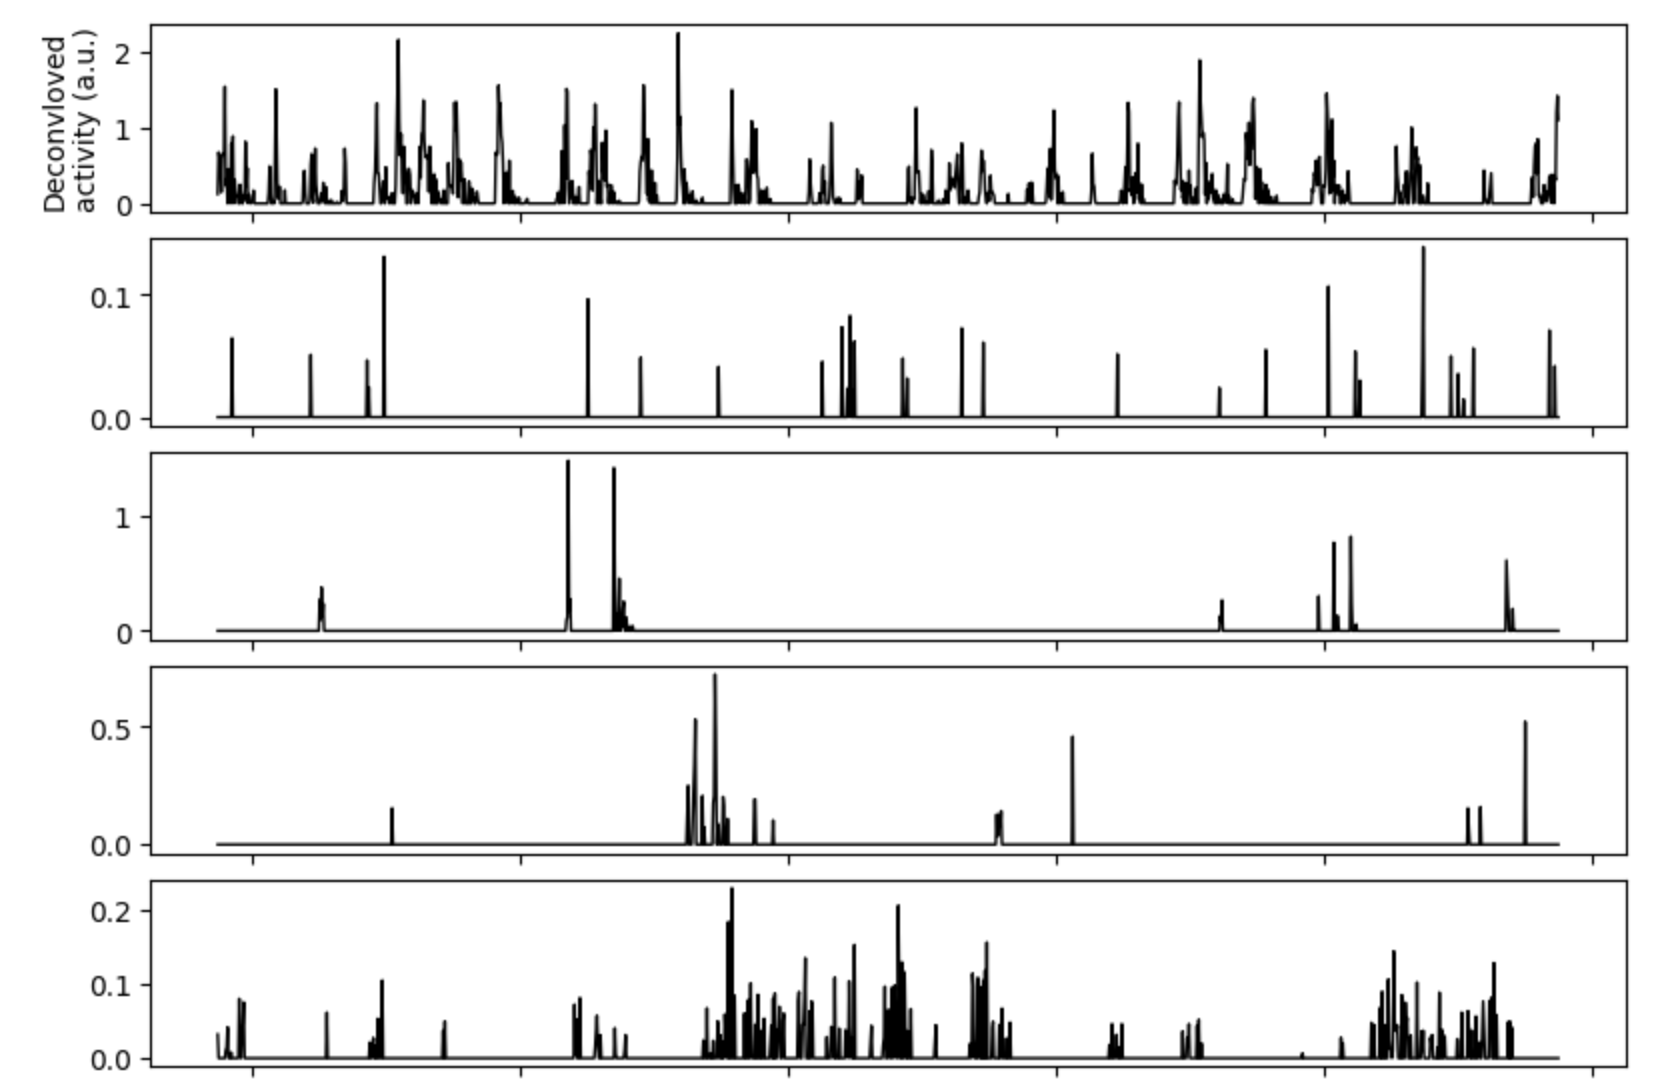
\includegraphics[width=0.75\linewidth]{neural_activity.png}
  \caption{Inferred neural spike activity from neuropixels }
  \label{fig:your-label}
\end{figure}


\section{Challenges:}
\subsection{Non-Smoothness}
The neural spiking data is non-smooth, and hence cannot be directly modeled via a deterministic ordinary differential equation. Specifically, we cannot assume the existence of higher-order time derivatives, and spikes might cause problems in learning an ode model. 

\subsection{Dimensionality}
In addition to non-smoothness, the dimensionality of the dataset is high as it involves recording neural activity from multiple neurons simultaneously. High-dimensional data poses challenges in terms of computation, visualization, and interpretation. 


\section{Expected outcomes}

We expect that our methods will enable us to extract meaningful information from neuron recordings, and to uncover the underlying network structure and dynamics of the brain. By analyzing the temporal correlations and causal interactions between neurons, we hope to gain insights into the neural mechanisms that give rise to complex behaviors and cognitive processes. We also anticipate that our methods will have broad applicability to other fields of science and engineering that involve the analysis of complex dynamical systems.

\section{Conclusion}

In summary, this research project aims to develop methods for estimating the dynamics of the brain from neuron recordings, and to apply these methods to real data. We anticipate that our methods will provide valuable insights into the dynamics of the brain, and will have broad applicability to other fields of science and engineering.

\section{Appendix}
\subsection{PCA}
In this study, Principal Component Analysis (PCA) was employed to reduce the dimensionality of neural spiking data obtained from \cite{tseng2022shared}. The dataset comprises recordings of neural activity originating from various regions of the mouse cortex during a navigation task. 
\\


\begin{figure}[htbp] % You can adjust the placement options (htbp) as needed
  \centering
  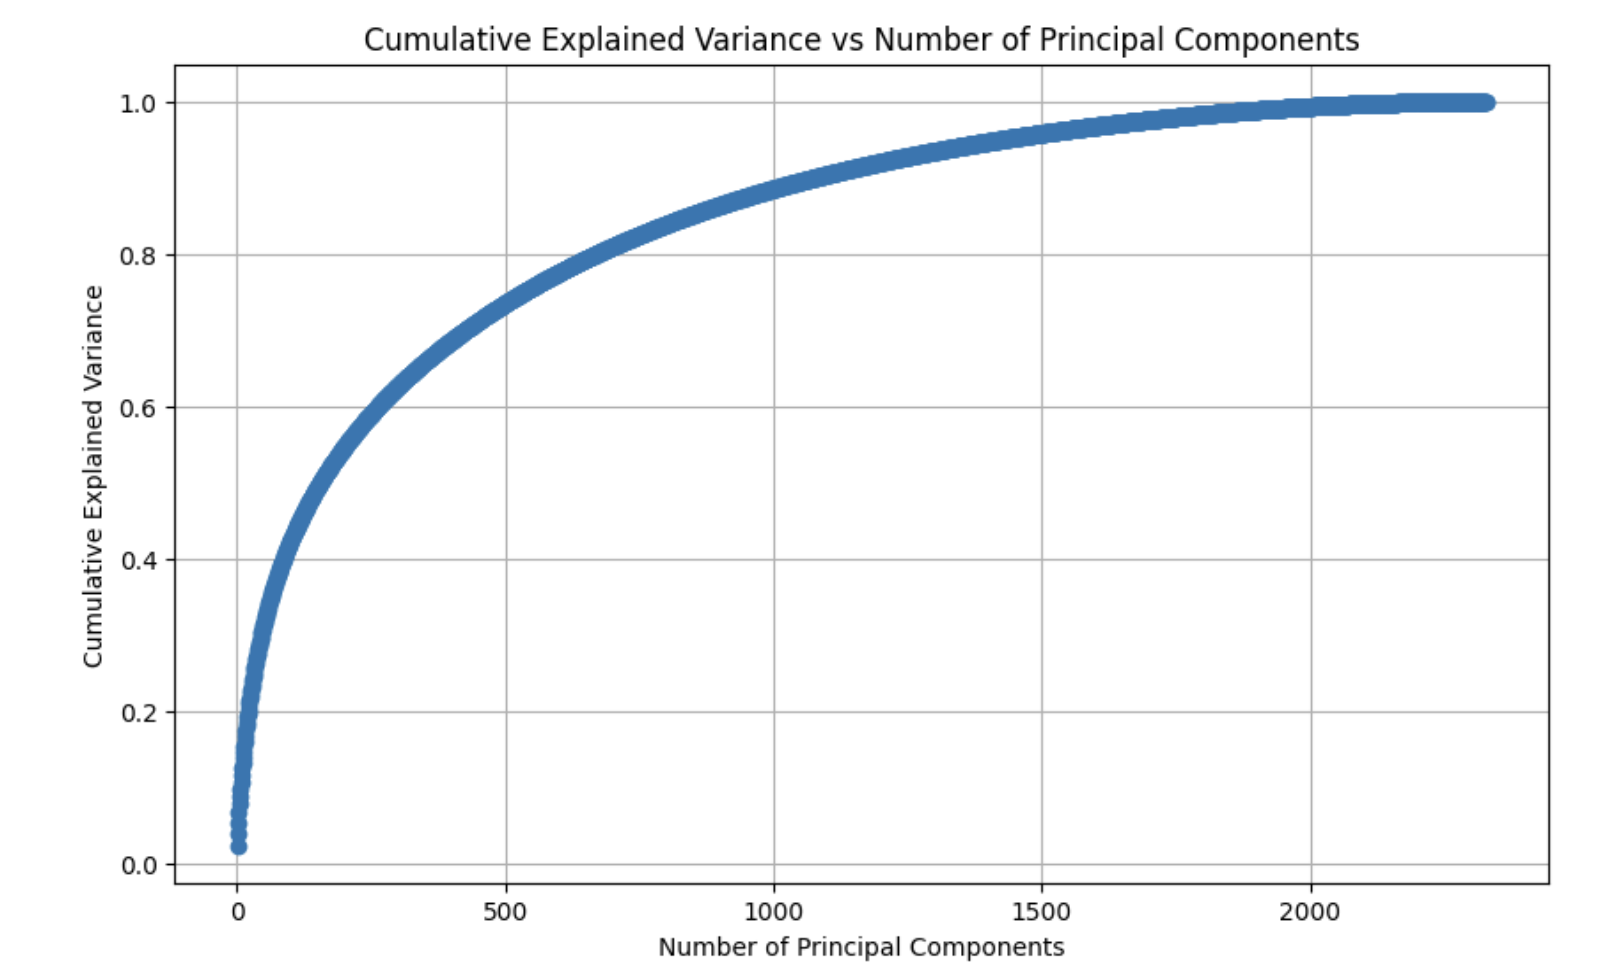
\includegraphics[width=0.75\linewidth]{explained_variance.png}
  \caption{Cumulative Explained Variance }
  \label{fig:your-label}
\end{figure}

\begin{figure}[htbp] % You can adjust the placement options (htbp) as needed
  \centering
  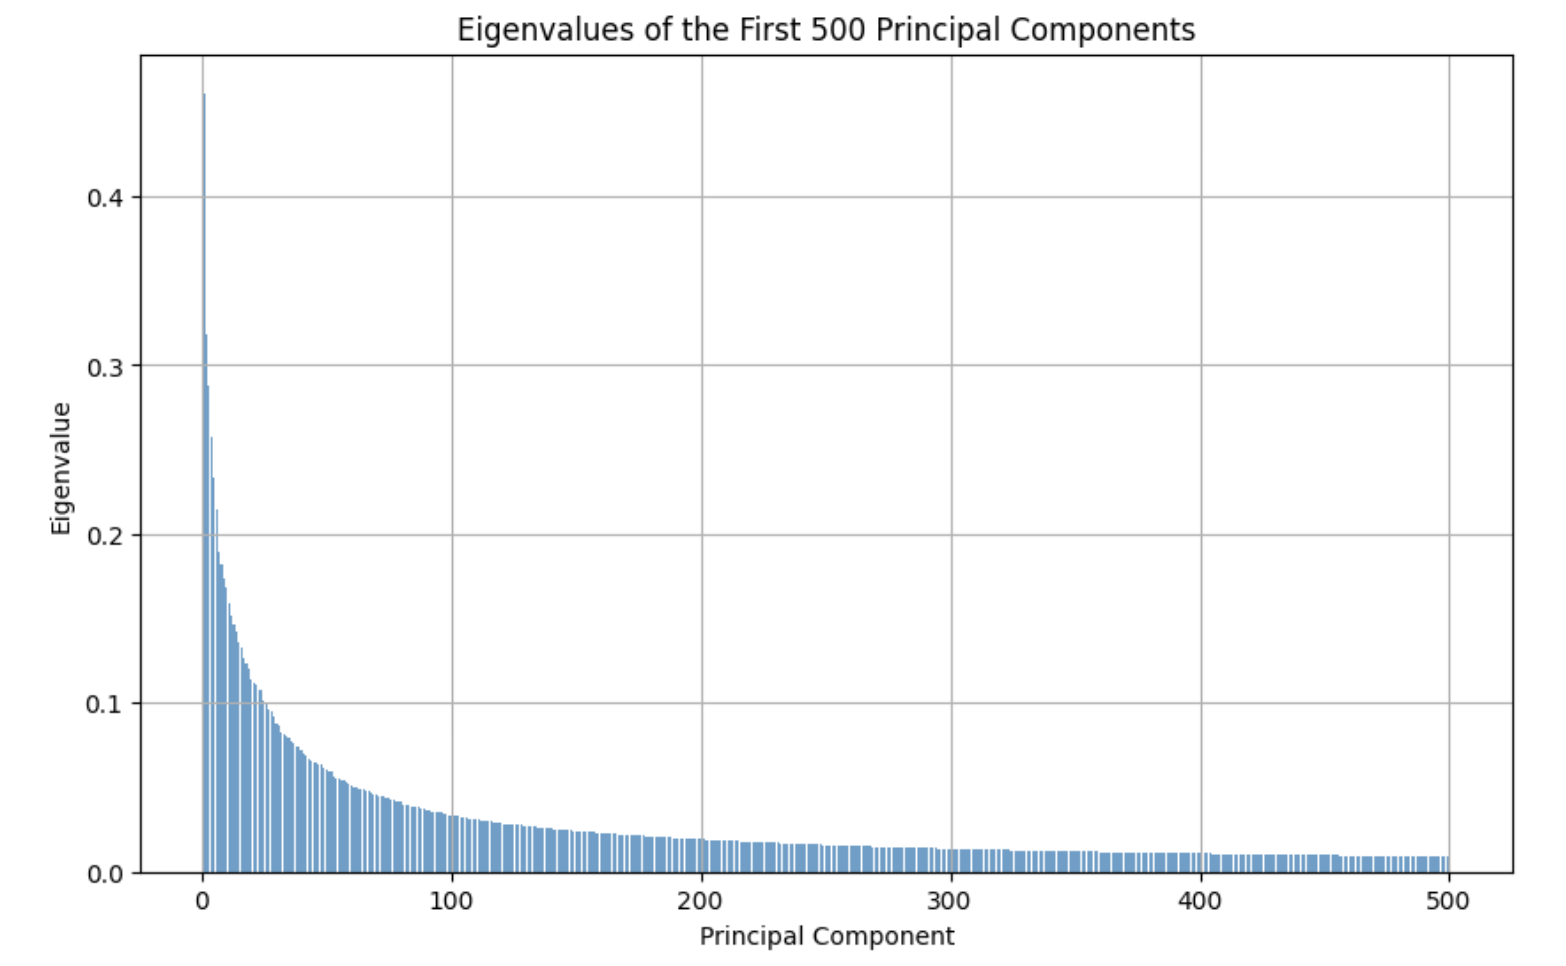
\includegraphics[width=0.75\linewidth]{eigenvalue_plot.png}
  \caption{Eigenvalue Decay }
  \label{fig:your-label}
\end{figure}
\newpage
\bibliographystyle{plain} 
\bibliography{references}
\end{document}